To get good results some experiments were conducted first to find the best possible architecture. After that, the obtained results were analyzed on in regard of the different corruption types.

\section{Experiments}

\subsection{Corruption Rate}

\begin{table}[t]
\begin{subtable}{\linewidth}\centering
{\begin{tabular}{ | r | r |r | r | r | r |r | }
  \hline
  & NC & MS & MB & VAR & RET & SL \\
  \hline
  \hline
  100\% & 60.0 & 64.0 & 48.2 & \textbf{37.3} & 54.3 & 26.7 \\
  \hline
  75\% & \textbf{70.4} & \textbf{71.8} & \textbf{51.3} & 34.4 & \textbf{55.1} & \textbf{42.6} \\
  \hline
  50\% & 62.0 & 61.2 & 43.7 & 25.0 & 47.4 & 26.1 \\
  \hline
  25\% & 67.9 & 65.6 & 41.6 & 19.6 & 50.3 & 33.3 \\
  \hline
\end{tabular}}
\caption{Performance of models with different corruption rates.}\label{corruption_rate_table}
\end{subtable}
\newline
\vspace*{5mm}
\newline
\begin{subtable}{\linewidth}\centering
{\begin{tabular}{ | m{3cm} | r | r | r | r | r | r | }
  \hline
  & NC & MS & MB & VAR & RET & SL \\
  \hline
  \hline
  with attention & \textbf{70.4} & \textbf{71.8} & \textbf{51.3} & \textbf{34.4} & \textbf{55.1} & \textbf{42.6} \\
  \hline
  without attention & 0.0 & 0.0 & 0.0 & 0.0 & 0.0 & 0.0 \\
  \hline
  without attention, input reversed & 0.0 & 0.0 & 0.0 & 0.0 & 0.0 & 0.0 \\
  \hline
\end{tabular}}
\caption{Performance of models with or without an attention mechanism.}\label{attention_mechanism_table}
\end{subtable}
\newline
\vspace*{5mm}
\newline
\begin{subtable}{\linewidth}\centering
{\begin{tabular}{ | l | r | r | r | r | r | r | }
  \hline
  & NC & MS & MB & VAR & RET & SL \\
  \hline
  \hline
  LSTM & \textbf{70.4} & \textbf{71.8} & \textbf{51.3} & \textbf{34.4} & \textbf{55.1} & \textbf{42.6} \\
  \hline
  GRU & 0.2 & 0.2 & 0.2 & 0.2 & 0.2 & 0.2 \\
  \hline
  vanilla RNN & 0.0 & 0.0 & 0.0 & 0.0 & 0.0 & 0.0 \\
  \hline
\end{tabular}}
\caption{Performance of different RNN types.}\label{rnn_type_table}
\end{subtable}
\caption{Evaluation of the performance of the models on the test set with different corruptions: uncorrupted (NC), missing semicolon (MS), missing bracket (MB), misspelled variable (VAR), wrong return type (RET) and line switch (SL).}
\end{table}

Because the source sequence and target sequence are almost the same and the errors are self-introduced, it is an interesting question what the optimal corruption rate for the input is. To test this the model was trained with four different corruption rates, 100\%, 75\%, 50\% and 25\%. The results can be seen in Table \ref{corruption_rate_table}.

For almost all corruptions the model trained with a corruption rate of 75\% posted the best result. The models with lower percentages didn't pick up on the errors as well while the model with the 100\% corruption rate didn't get as good an understanding of when the code is correct. In general, the model learned to correct all of the introduced errors. It performed especially well when inputting a sequence missing a single semicolon which is of course also the simplest task to solve. However, the model was also able to correct the other errors reasonably well. A missing bracket or an incorrect return type were corrected most of the time while the model had a little more trouble correcting a misspelled variable or realigning switched lines. A more detailed analysis of the different error types is given in Section \ref{error_analysis}.

What is also interesting to see is how well the model performed on uncorrupted sequences. Even the model with 100\% corruption rate, i.e. which never got an uncorrupted sequence as input, managed to not introduce any new errors into an uncorrupted sequence most of the time. This indicates that the model obtains some understanding of the input and how code works and only corrects where necessary.

Going forward all experiments were done with a corruption rate of 75\% and the error analysis was also done on the results of this model.

\subsection{Attention Mechanism}

\begin{figure}[p]
\centering
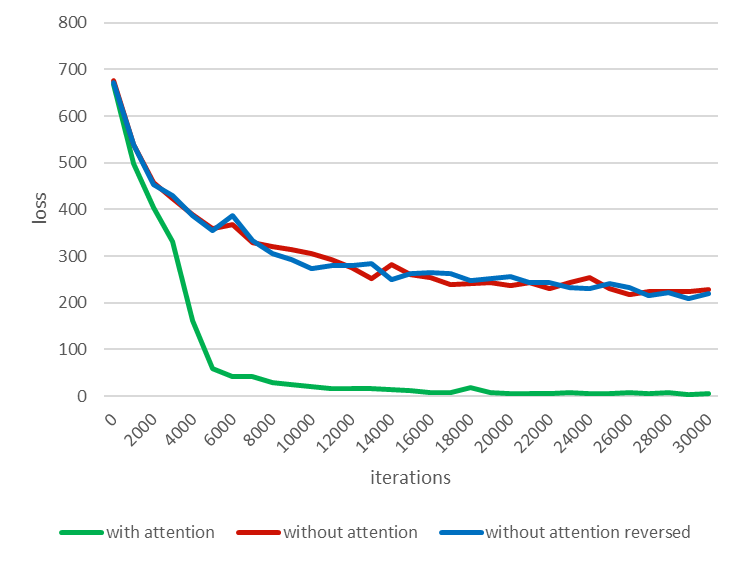
\includegraphics[width=0.9\linewidth]{attention_chart}
\caption{The training loss of models with or without an attention mechanism as a function over iterations.}
\label{attention_chart}
\end{figure}

Another interesting question is if the attention mechanism is essential for the model. After all, it increases complexity and training duration. To test this, the model was twice trained without the attention mechanism on top of the decoder, once with the same input the regular model got and once with the input reversed. The reversion of the input is a technique proposed in \cite{seq2seq}, the idea being to introduce more short-term dependencies while the average distance of the dependencies stays the same. This is not necessary for the regular model because the attention mechanism allows the model to take a peek of the encoder state many timesteps ago.

The experiment revealed the attention mechanism to be an essential part of the model because the models without the mechanism weren't able to solve the given task at all (see Table \ref{attention_mechanism_table}). These models never learned to repeat the input sequence probably because they couldn't pass all information from the encoder to the decoder in a single vector.

For the first couple of thousand iterations, all models learned roughly the same things, namely the general structure of the desired output. The models would start to begin the output sequence with \texttt{public ...(...)\{} and end it with \texttt{\}<eos>}. In between, they added mostly snippets that look like code but don't make any sense. However, after about 4,000 iterations the model with the attention mechanism learned to utilize the mechanism to its full potential and started repeating the input sequence. This resulted in rapid performance improvement. The training loss of the different configurations as a function over iterations can be seen in Figure \ref{attention_chart}.

The reversion of the input sequence helped the model to learn a little bit faster but overall it made almost no difference. The model was still not able to solve the task.

\subsection{RNN type}

\begin{figure}[p]
\centering
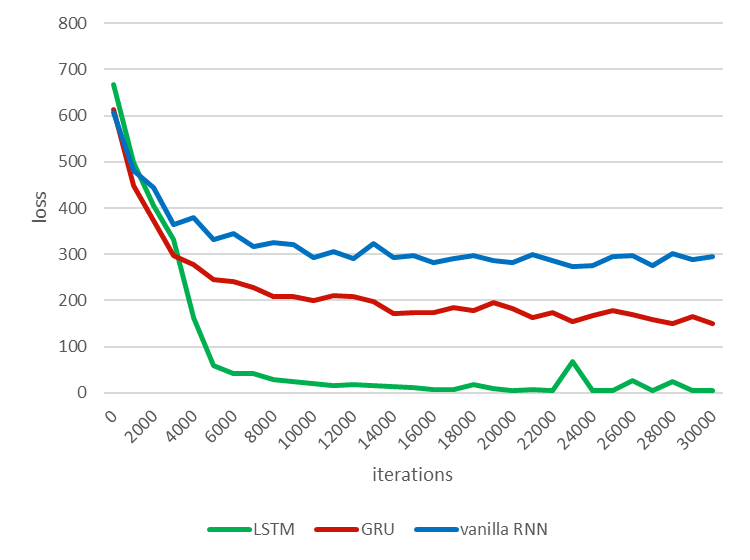
\includegraphics[width=0.9\linewidth]{cell_type_chart}
\caption{The training loss of different recurrent network types as a function over iterations.}
\label{cell_type_chart}
\end{figure}

In Subsection \ref{rnn_types} three types of RNNs were listed: vanilla RNNs, LSTMs and GRUs. To test which type works best for the given task, a model was trained for each RNN type. The training loss of the models as a function over iterations can be seen in Figure \ref{cell_type_chart}. The evaluation on the test set can be found in Table \ref{rnn_type_table}.

As could be expected the vanilla RNN performed the worst. As explained earlier, these networks have trouble with long-range dependencies and struggle with the problem of vanishing gradients. The vanilla RNN is also the simplest type and thus the one with the least amount of trainable parameters.

More surprising was the performance gap between the GRU and the LSTM, because recent research suggests that these two network types have a comparable performance \cite{lstm_vs_gru}. However similar to the models without the attention mechanism, the GRU network never fully learns to repeat the input sequence. One possible explanation for this is the fewer parameters of the GRU. An LSTM computes three gates at each timestep while also passing a memory vector to the next timestep. A GRU only has two gates and doesn't have a second vector in addition to the hidden state vector. Because the 256 units per layer are relatively few the lack of trainable parameters could prevent the GRU from learning as well as the LSTM.

\section{Error analysis}
\label{error_analysis}

In this section, the performance of the model on uncorrupted input and on each of the five corruptions is analyzed. For examples from the test set see appendix \ref{showcase}.

\subsection{Uncorrupted}

The model works reasonably well on uncorrupted input with a 70.4\% success rate. However, it is still of interest to see, what kind of errors are introduced by the network, i.e. where and why it gets confused. One mistake the model makes repeatedly is a "one-off error". Here the model would output a wrong character whose ASCII encoding is just by one off of the encoding of the correct character. For example, sometimes an asterisk whose ASCII encoding is 42 is output while the correct character would be a plus (ASCII encoding 43). If the results of the model are evaluated with a tolerance for these errors (i.e. if a character is just by one off it is not seen as an error), the accuracy of the model increases to 79.6\%. That's an almost 10\% performance increase and the model should be able to learn to avoid these mistakes with more training.

Another common error is the random switching of lines. An additional 4.8\% of the test set would have been correct if it wasn't for an incorrect line switch. This suggests that the model didn't learn to correct this corruption that well. This problem is elaborated further in Subsection \ref{switch_analysis}.

The last thing that was noticeable in the test set was that sometimes the model would get stuck in some kind of loop and output some parts or lines of the input sequence multiple times. This is something that can often be observed in the early stages of training which suggests that the model should be able to avoid these mistakes with more training.

\subsection{Missing Semicolon}

The same mistakes that were observed on uncorrupted input of course also apply to the correction of corrupted input. The correction of a missing semicolon should be the easiest error to correct and while the accuracy is already good with 71.8\% it is also worth to look at the results of an evaluation with the same "one-off tolerance" as in the evaluation of the uncorrupted results in which case the model is 81.7\% accurate. In addition to that 3.2\% of the time, an error was introduced by an incorrect line switch.

What's also interesting to see is that the output contains the correct number of semicolons in 97.0\% of the time. This means that the absence of a semicolon is detected and corrected nearly every time, there are just new mistakes that are introduced by the model into the output.

\subsection{Missing Brackets}

The main advantage of LSTMs is their ability to remember long-range dependencies which should be very useful for detecting and correcting missing brackets but the test accuracy of 51.3\% seems to contradict this assumption. However, a closer look at the results reveals that the task of inserting a missing bracket isn't that trivial. Consider the following example:

\begin{lstlisting}[style=inline]
public int addint a, int b){
  int sum = a + b;
  return sum;
}
\end{lstlisting}

Here the opening bracket between the method name and the parameters was removed. The task for the model is now to not only detect that a bracket is missing but also to find the correct spot to reinsert it which is even more difficult when there is no white space indicating the location of the missing bracket.

To see how many times the missing bracket was detected the test results were evaluated to look if the brackets in the output were balanced, meaning if every opening bracket had a closing counterpart and vice versa. The evaluation showed that the model managed to balance the brackets in 77.2\% of the time. In addition to that, the brackets were also correctly nested 76.9\% of the time which indicates that the model did learn the close open brackets very well.

\subsection{Misspelled Variable}

\begin{figure}[t]
\centering
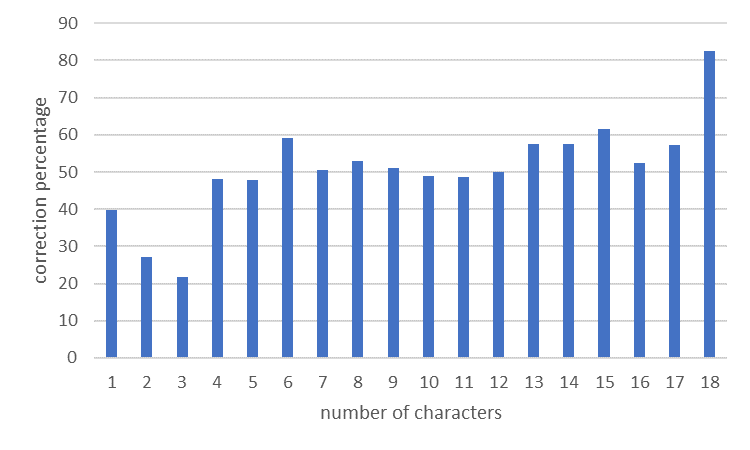
\includegraphics[width=0.9\linewidth]{variables_chart}
\caption{Correction percentages for variables of different lengths. Only lengths with more than 10 examples were considered.}
\label{variables_chart}
\end{figure}

The correction of misspelled variables was the most difficult corruption to correct for the model with an overall accuracy of 34.4\%. However when the test results are evaluated to see if the output contained the correct number of occurrences of the variable either all of them correctly spelled or all of them misspelled, the accuracy increases to 45.6\%. This includes examples where the variable was corrected but some other error was introduced to the sequence and examples where the model corrected the wrong occurrence of the variable, i.e. it corrected the variable in the declaration to conform to the introduced misspelling later in the sequence. The latter of course also result in correct code because the variable is named consistently but it is not how the model is intended to correct variables.

The accuracy of the model was also evaluated in regard to the length of the variable name. These results can be found in Figure \ref{variables_chart}. As could be expected the model struggles with variables of shorter length. This suggests that the network looks for similar patterns in the sequence to determine if a variable is misspelled and then corrects it accordingly, which is, of course, easier to do if the variable name is longer. The only big exception are one-character variables but this most likely stems from the fact that these variables have a simpler corruption pattern because there are no two characters that can be switched and the deletion of a random character doesn't serve as well so the misspelling is always an additional character that has to be removed.

\subsection{Wrong Return Type}

\begin{table}[t]
\centering
\begin{tabular}{ | l | r | }
  \hline
  Return Type & Accuracy \% \\
  \hline
  \hline
  byte(1) & 100.0 \\
  \hline
  State(15) & 86.7 \\
  \hline
  int(447) & 70.5 \\
  \hline
  void(5022) & 68.2 \\
  \hline
  String(321) & 60.8 \\
  \hline
  IFigure(284) & 44.7 \\
  \hline
  Collection(24) & 33.3 \\
  \hline
  boolean(168) & 14.3 \\
  \hline
  Double(82) & 0.0 \\
  \hline
  Session(1) & 0.0 \\
  \hline
\end{tabular}
\caption{Some return types and their correction percentages. The number in brackets indicates the number of occurrences of this type in the test set.}
\label{return_type_selection_table}
\end{table}

As discussed in Subsection \ref{corruption} it is not always possible to derive the correct return type from a method. Sometimes there is no indication of the correct type or the return type is specified as a superclass or interface of the object that is actually returned. In regard of this, the 55.1\% accuracy scored by the model is pretty good. To analyse this result further the model was evaluated to see which types it was able to correct and with which it struggled. A selection of these results can be found in Table \ref{return_type_selection_table}.

The accuracy for different data types varies greatly. There are some data types (alas not many) that the model never manages to correct. This can have different causes for example as mentioned it could be impossible to derive the correct return type or in the case of \texttt{Double} the model can also be confused by the distinction of the primitive data type \texttt{double} and its object wrapper \texttt{Double}. In the case of a \texttt{boolean} return type, there is also the additional difficulty that often no variable of type \texttt{boolean} is returned but rather a statement that resolves to a \texttt{boolean} value, e.g. \texttt{return i == 1;}.

Even though the model generally scores better on examples that occur more often, it can also be seen that this is no necessity for the model to derive the correct return type. For example, \texttt{byte} only occurs once in the test set and probably not much more in the training data and the model still managed to derive the correct return type for the method.

\subsection{Line Switch}
\label{switch_analysis}

\begin{table}[t]
\centering
\begin{tabular}{ | l | r | r | r | }
  \hline
  \(\leftrightarrow\) & VD & MI & AS \\
  \hline
  \hline
  VD & - & 53.3 & \textbf{59.3} \\
  \hline
  MI & 0.0 & - & 13.0 \\
  \hline
  AS & 0.0 & 9.8 & - \\
  \hline
\end{tabular}
\caption{The correction percentages for different line switches. The rows indicate the type of the first line and the columns the type of the second line. There are three possible types: variable declaration (VC), method invocation (MI) or assignment (AS). Only lines of different types were switched.}
\label{switch_table}
\end{table}

At first sight, the performance of the model on the switched lines corruption appears to be pretty good with 42.6\%. However, observations from the previous subsections suggest that the model still gets confused with some line switches. For this purpose, the test results were evaluated with regard to the type of the switched lines. The scores can be found in Table \ref{switch_table}.

It quickly becomes apparent that the model only really learns to correct line switches where the first line is a variable declaration. These switches mostly produce semantic errors rather than logic ones because often the declared variable is used in the other line and therefore before it was declared after the switch. For example the error in:

\begin{lstlisting}[style=inline]
public int add(int a, int b){
  sum = a + b;
  int sum;
  return sum;
}
\end{lstlisting}

\noindent is a semantic one and not a logic one. Furthermore by going through the test results, one can see that the other switches often don't produce any error at all (examples can be found in Appendix \ref{showcase}). Unfortunately, it is not possible to evaluate the percentage of introduced errors quantitatively because there would be no need to train a model on the task of logic error detection if it could already be done reliably.

Nevertheless, it is reasonable to draw the conclusion that the model gets confused by the line switches with low correction accuracy because it cannot figure out when and how they occur. This is probably the reason for the random line switches discussed in previous subsections. These low accuracy switches are also the ones that are not very likely to produce an error.
